% =====================================================================
%  Informe Tarea 2 - EI-4419 - GR09
%  Documento completo en un solo archivo.
%  Figuras: ../matlab/figuras_diseno/ (diseno_compensador.m) y
%           ../resultados_matlab/ (scripts del integrante 1 y 3)
% =====================================================================
\documentclass[journal,twocolumn]{IEEEtran}
\usepackage[utf8]{inputenc}
\usepackage[T1]{fontenc}
\usepackage[provide=*,spanish]{babel}
\addto\captionsspanish{\renewcommand{\figurename}{Figura}\renewcommand{\tablename}{Tabla}}
\usepackage{amsmath,amssymb,booktabs,cite,tikz,tabularx,array,graphicx}
\usepackage{microtype,xurl,flafter,balance}
\newcolumntype{L}{>{\raggedright\arraybackslash}X}
\newcommand{\tableformat}{\footnotesize\setlength{\tabcolsep}{3pt}\renewcommand{\arraystretch}{1.15}}
\setlength{\emergencystretch}{1em}
\usetikzlibrary{arrows.meta,positioning}
\graphicspath{{../matlab/figuras_diseno/}{../resultados_matlab/}}
% Marca de texto pendiente (borrar todos los \pendiente antes de entregar)
\newcommand{\pendiente}[1]{\textit{[Pendiente: #1]}}
\begin{document}
\title{Control de temperatura de una celda Peltier: análisis proporcional y diseño de un compensador PI con anti-windup}
\author{Carlos Andrés Castro Villegas, Victoria Slyn Cerdas López y Jiahui Zhong Xie%
\thanks{Los autores pertenecen a la Escuela de Ingeniería Electrónica del Instituto Tecnológico de Costa Rica. Trabajo presentado en el curso EI-4419 Análisis y Control de Sistemas Lineales, Grupo 9, II semestre de 2026.}}
\maketitle
\begin{abstract}
Se diseña un lazo de control para la temperatura del bloque frío de la planta termoeléctrica de la Tarea~1, formada por una celda TEC1-12706, un bloque de aluminio y un disipador ventilado. Primero se estudia un controlador proporcional: el lazo lineal es estable para toda ganancia positiva, pero el error en estado estable y el rechazo de perturbaciones exigen ganancias que superan el esfuerzo de control permitido. Además, la curva estática de la planta muestra que con más de $2.42\,\mathrm A$ la corriente calienta el bloque, por lo que la salida del controlador se limita a $2\,\mathrm A$. Se definen ocho especificaciones cuantitativas a partir del rango de $2$ a $8\,^\circ\mathrm C$ de la cadena de frío y de la resolución de un sensor DS18B20. Se selecciona un PI con el cero sobre el polo lento de la planta ($T_i=116.2\,\mathrm s$) y $K_c=0.75\,\mathrm{A/K}$, con anti-windup por integración condicional. El modelo lineal predice error nulo, asentamiento en $158.6\,\mathrm s$ y margen de fase de $98.7^\circ$; en el arranque no lineal el bloque llega a $5\pm0.5\,^\circ\mathrm C$ en $117\,\mathrm s$ sin bajar de $4.87\,^\circ\mathrm C$. \pendiente{completar con los resultados de Simscape y la comparación.}
\end{abstract}
\begin{IEEEkeywords}Celda Peltier, control proporcional, controlador PI, anti-windup, especificaciones de diseño, regulación térmica.\end{IEEEkeywords}

% Responsable: Integrante 3 (tarea 3.2 del plan)
\section{Introducción}
\pendiente{contexto de la regulación térmica con celdas Peltier, objetivo de la Tarea~2 (continuación de la Tarea~1) y organización del artículo.}

% Responsable: Integrante 3 (tarea 3.2 del plan)
% Resumir de la Tarea 1: componentes (con su fuente en los cuadros de
% parámetros), modelo no lineal, espacio de estados, G(s) e imagen del
% modelo Simscape (recomendación del profesor).
\section{Descripción del sistema}
\pendiente{celda TEC1-12706 \cite{hb}, bloque de aluminio, disipador y ventilador de $400\,\mathrm{LFM}$; tabla de parámetros con la fuente de cada componente; diagrama funcional de bloques.}

\section{Modelo de la planta}
\pendiente{ecuaciones no lineales, punto de operación ($T_{b0}=5\,^\circ\mathrm C$, $I_0=1.19\,\mathrm A$), espacio de estados y función de transferencia de la Tarea~1; imagen del modelo Simscape con su fuente.}

% Responsable: Integrante 1 (tareas 1.1 y 1.2 del plan)
\section{Implementación del lazo cerrado}\label{sec:lazo}
\subsection{Variable controlada y referencia}
Se conserva la planta termoeléctrica de la Tarea 1, con corriente $I$ como entrada y temperatura $T_b$ del bloque frío como salida. Se adopta como objetivo nominal $T_b=5\,{}^\circ\mathrm C$, ambiente de $25\,{}^\circ\mathrm C$ y flujo de aire de $400\,\mathrm{LFM}$. El punto de operación guardado en el proyecto es
\begin{align}
 I_0&=1.190149\,\mathrm A, &T_{b0}&=278.15\,\mathrm K,\\
 T_{h0}&=304.101077\,\mathrm K, &R_{HA}&=1.29\,\mathrm{K/W}.
\end{align}
La referencia representa regulación de una carga térmica, por lo que resulta físicamente coherente con la salida modelada. Para estudiar el seguimiento local se propone un cambio de $5$ a $4\,{}^\circ\mathrm C$ en $t=20\,\mathrm s$. El arranque se estudia por separado, con ambas masas inicialmente a $25\,{}^\circ\mathrm C$ y referencia constante de $5\,{}^\circ\mathrm C$; esta condición está alejada de la linealización.

\subsection{Convención de signo y límites}
Como la ganancia de pequeña señal de la planta es negativa, se define
\begin{align}
 e(t)&=T_{b,\mathrm{med}}(t)-T_{\mathrm{ref}}(t),\label{eq:error}\\
 I(t)&=\operatorname{sat}_{[0,\,2]}\{I_0+K_p e(t)\}.\label{eq:leyP}
\end{align}
Una temperatura superior a la referencia produce un incremento de corriente para $K_p>0$. El sesgo $I_0$ mantiene la corriente necesaria en el equilibrio nominal. El límite superior de $2\,\mathrm A$ se justifica en la Sección~\ref{sec:limite}. La planta física recibe corriente absoluta; la representación lineal recibe $\Delta I=I-I_0$. Las temperaturas internas se expresan en kelvin y se convierten a grados Celsius para la medición y las figuras. La Figura~\ref{fig:lazoP} muestra el lazo resultante.
% NOTA para el integrante 1: los ensayos se prepararon con Imax = 6.4 A.
% Cambiar Imax a 2.0 en parametros_ensayos.mat y repetir (ver Sección límite).

\begin{figure}[!tbp]
\centering
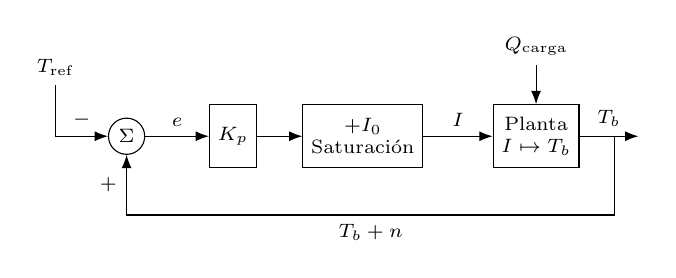
\begin{tikzpicture}[>=Latex,font=\scriptsize,
 b/.style={draw,align=center,minimum height=8mm,inner sep=3pt}]
\node[draw,circle,inner sep=2pt] (e) at (0,0) {$\Sigma$};
\node[b] (k) at (1.35,0) {$K_p$};
\node[b] (s) at (3.0,0) {$+I_0$\\Saturación};
\node[b] (p) at (5.2,0) {Planta\\$I\mapsto T_b$};
\node (y) at (6.5,0) {};
\draw[->] (e)--node[above]{$e$}(k);
\draw[->] (k)--(s);
\draw[->] (s)--node[above]{$I$}(p);
\draw[->] (p)--node[above]{$T_b$}(y.center);
\draw[->] (6.2,0)--(6.2,-1.0)--node[below]{$T_b+n$}(0,-1.0)--node[left]{$+$}(e);
\draw[->] (-0.9,0.65)node[above]{$T_{\rm ref}$}--(-0.9,0)--node[above]{$-$}(e);
\draw[->] (5.2,0.9)node[above]{$Q_{\rm carga}$}--(p);
\end{tikzpicture}
\caption{Lazo de acción inversa con control proporcional. El ruido $n$ se suma en la medición; la perturbación térmica entra en la planta. Fuente: elaboración propia.}
\label{fig:lazoP}
\end{figure}

La implementación propuesta utiliza dos modelos. La red Simscape se reutiliza de la Tarea 1. En la representación lineal se conservan los dos estados térmicos para incorporar condiciones iniciales, una entrada adicional de calor y la temperatura caliente. Una rama con la función de transferencia $G(s)$ verifica la salida de pequeña señal desde equilibrio. Así se mantiene el mismo modelo lineal de la tarea previa y se evita atribuir a una función de transferencia con condiciones iniciales nulas un arranque que no describe por sí sola.

% Responsables: Integrante 1 (análisis base) e Integrante 2 (lugar de las
% raíces, perturbaciones y límite de corriente)
\section{Análisis del controlador proporcional}\label{sec:P}
La función de transferencia nominal es
\begin{equation}
G(s)=\frac{-0.291898s-0.00424337}{s^2+0.0563263s+0.000410735}.\label{eq:G}
\end{equation}
Con la convención de la ecuación~\eqref{eq:error}, el lazo equivale a una realimentación negativa sobre la planta de acción inversa
\begin{equation}
G_p(s)=-G(s)=\frac{0.2919\,s+0.004243}{s^2+0.05633\,s+0.0004107}\ \left[\mathrm{K/A}\right].\label{eq:Gp}
\end{equation}
Sin saturación, la transferencia de referencia a salida y el polinomio característico son
\begin{align}
 T_P(s)&=\frac{-K_pG(s)}{1-K_pG(s)},\\
 D_P(s)&=s^2+(0.0563263+0.291898K_p)s\notag\\
 &\quad +(0.000410735+0.00424337K_p).\label{eq:carP}
\end{align}
Los coeficientes son positivos para $K_p>0$ y el criterio de segundo orden establece estabilidad del modelo lineal nominal. Esta conclusión es local: no demuestra regulación global con saturación ni con variaciones grandes de temperatura.

La Figura~\ref{fig:lgrP} muestra el lugar de las raíces: una rama va del polo $-0.0086\,\mathrm{s^{-1}}$ al cero $-0.0145\,\mathrm{s^{-1}}$ y la otra parte de $-0.0477\,\mathrm{s^{-1}}$ hacia $-\infty$. Los polos siempre son reales, por lo que el modelo lineal no presenta sobrepaso con ningún $K_p$.

\begin{figure}[!tbp]\centering
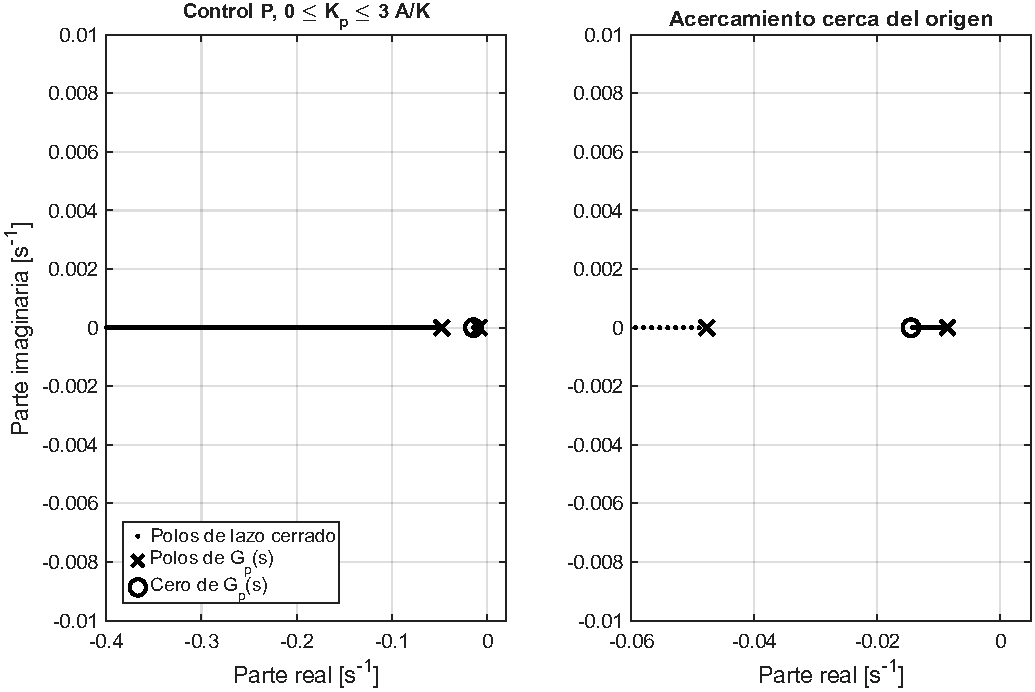
\includegraphics[width=\columnwidth]{lgr_P}
\caption{Lugar de las raíces de $K_pG_p(s)$ para $0\le K_p\le3\,\mathrm{A/K}$. A la derecha, acercamiento a la región cercana al origen. Fuente: elaboración propia con MATLAB R2025a.}\label{fig:lgrP}
\end{figure}

Para un escalón de referencia de magnitud $|\Delta r|$, la magnitud del error estacionario lineal es
\begin{equation}
 |e_{ss}|=\frac{|\Delta r|}{1-K_pG(0)}\simeq\frac{|\Delta r|}{1+10.331K_p}.\label{eq:essP}
\end{equation}
El error que usa el controlador es $T_b-T_{\rm ref}$; en las tablas se reporta también su magnitud para facilitar la comparación. La fórmula anterior corresponde a un cambio de referencia respecto del equilibrio. En un arranque que retorna al punto nominal, el sesgo $I_0$ puede permitir error final cero si el sistema converge y no recibe perturbaciones constantes.

Las perturbaciones se tratan de la misma forma. Con los balances de la Tarea~1, un cambio de la temperatura ambiente llega a la salida por $G_d(s)=\Delta T_b/\Delta T_{\rm amb}$, con $G_d(0)=0.918\,\mathrm{K/K}$, y una carga de calor $Q$ aplicada al bloque llega por $G_q(s)=(C_Hs+g_H)/D_G(s)$, con $G_q(0)=2.51\,\mathrm{K/W}$. Para un escalón de $+5\,\mathrm K$ en $T_{\rm amb}$ y una carga de $2\,\mathrm W$, las desviaciones permanentes son
\begin{equation}
\Delta T_{b,ss}=\frac{4.59\,\mathrm K}{1+10.33\,K_p}\quad\text{y}\quad\Delta T_{b,ss}=\frac{5.02\,\mathrm K}{1+10.33\,K_p}.\label{eq:essD}
\end{equation}
La Tabla~\ref{tab:P_analitico} resume el comportamiento lineal para cinco ganancias. El error disminuye con $K_p$, pero solo se anula con ganancia infinita. Además, el esfuerzo de control inicial es $\Delta I(0^+)=K_p\,|\Delta T_{\rm ref}|$, porque $G_p(s)$ es estrictamente propia: reducir el error con ganancia aumenta proporcionalmente la corriente.

\begin{table}[!tbp]\centering
\caption{Desempeño lineal del control P (escalón de referencia de $1\,\mathrm K$, $+5\,\mathrm K$ en $T_{\rm amb}$ y carga de $2\,\mathrm W$).}\label{tab:P_analitico}
{\tableformat\setlength{\tabcolsep}{2.2pt}
\begin{tabular}{@{}ccccccc@{}}\toprule
\shortstack{$K_p$\\{[A/K]}} & \shortstack{$e_{ss}$\\{[\%]}} & \shortstack{$t_s$ (2\,\%)\\{[s]}} & \shortstack{$\Delta I_{\max}$\\{[A]}} & \shortstack{$\Delta T_{b,ss}$\\$T_{\rm amb}$ [K]} & \shortstack{$\Delta T_{b,ss}$\\2\,W [K]} & \shortstack{Polos\\{[$\mathrm{s^{-1}}$]}}\\\midrule
0.2 & 32.6 & 176.5 & 0.20 & 1.497 & 1.636 & $-0.1024$, $-0.0123$\\
0.5 & 16.2 & 106.7 & 0.50 & 0.744 & 0.813 & $-0.1889$, $-0.0134$\\
1.0 & 8.8 & 57.0 & 1.00 & 0.405 & 0.443 & $-0.3343$, $-0.0139$\\
2.0 & 4.6 & 11.5 & 2.00 & 0.212 & 0.232 & $-0.6259$, $-0.0142$\\
5.0 & 1.9 & 3.0 & 5.00 & 0.087 & 0.095 & $-1.5014$, $-0.0144$\\\bottomrule
\end{tabular}}
\par\smallskip\footnotesize Fuente: elaboración propia con \texttt{diseno\_compensador.m}.
\end{table}

El aumento de ganancia reduce el error, pero uno de los polos se aproxima al cero de la planta, situado cerca de $-0.01454\,\mathrm{s}^{-1}$. Deben examinarse tanto su posición como la amplitud de su contribución a la salida: un tiempo de subida corto no excluye una cola lenta.

En el arranque, el mando inicial solicitado es $I_0+20K_p$. Para las ganancias de $0.2$, $1$ y $5\,\mathrm{A/K}$ se obtienen $5.190$, $21.190$ y $101.190\,\mathrm A$, de modo que con el límite de $2\,\mathrm A$ las tres arrancan saturadas. El calentamiento Joule y el aumento de temperatura del disipador hacen necesario contrastar el arranque lineal con la planta no lineal.

\subsection{Límite útil de la corriente}\label{sec:limite}
La corriente máxima de la hoja de datos es $6.4\,\mathrm A$ \cite{hb}, pero ese valor no sirve como límite del controlador. La Figura~\ref{fig:limite} repite la curva estática de la Tarea~1: la temperatura de equilibrio del bloque alcanza su mínimo, $-1.05\,^\circ\mathrm C$, con $2.42\,\mathrm A$. Para corrientes mayores, el calor Joule y el calor que regresa desde el lado caliente dominan sobre el bombeo Peltier, de modo que más corriente \emph{calienta} el bloque. En esa zona la ganancia de la planta cambia de signo y la realimentación se vuelve positiva. Si el controlador puede llegar a $6.4\,\mathrm A$, en el arranque se satura arriba, el bloque se calienta, el error crece y la corriente se queda en el máximo: el bloque termina en $46.4\,^\circ\mathrm C$ (Figura~\ref{fig:arranque}). Por eso se limita la salida del controlador a $0\le I\le2.0\,\mathrm A$, un $17\,\%$ por debajo del mínimo de la curva.

\begin{figure}[!tbp]\centering
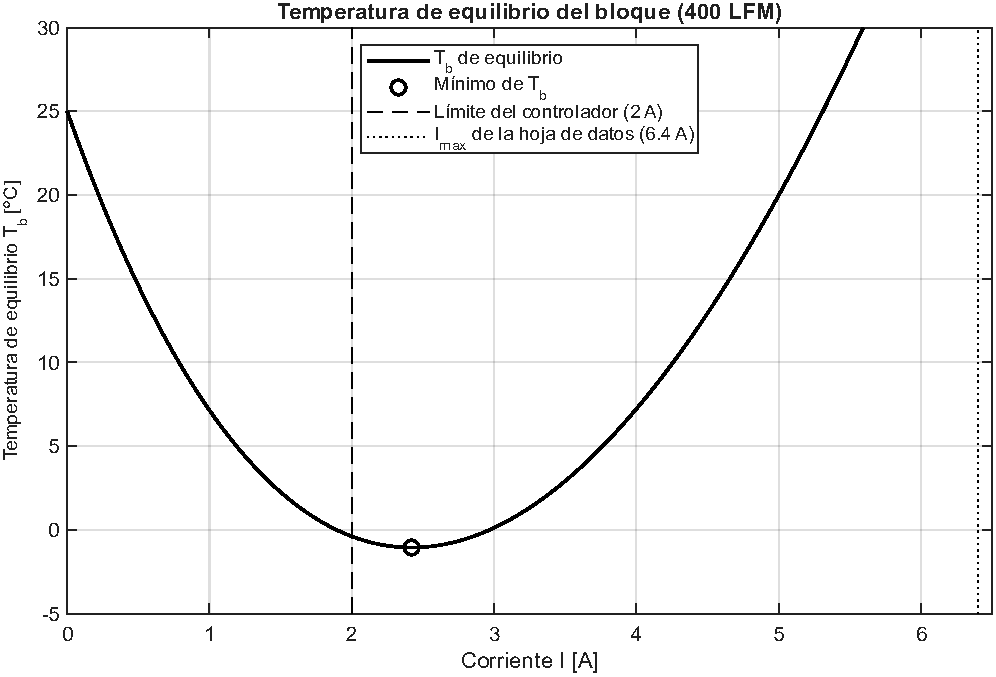
\includegraphics[width=\columnwidth]{limite_corriente}
\caption{Temperatura de equilibrio del bloque en función de la corriente con ventilador de $400\,\mathrm{LFM}$, límite elegido para el controlador ($2\,\mathrm A$) y corriente máxima de la TEC1-12706 ($6.4\,\mathrm A$) \cite{hb}. Fuente: elaboración propia a partir del modelo de la Tarea~1.}\label{fig:limite}
\end{figure}

% Responsable: Integrante 1 (tareas 1.3 a 1.5 del plan)
\section{Evaluación del desempeño}\label{sec:desempenoP}
\subsection{Pruebas y métricas}
Se prepararon cuatro pruebas de $1200\,\mathrm s$ para ambas plantas y $K_p=0.2$, $1$ y $5\,\mathrm{A/K}$: escalón de referencia, arranque desde ambiente, carga de calor de $2\,\mathrm W$ desde $300\,\mathrm s$ y ruido de medición desde ese mismo instante. La carga y el ruido se aplican en ensayos separados. El ruido tiene desviación estándar elegida de $0.05\,\mathrm K$ y muestras mantenidas durante $1\,\mathrm s$; representa una condición comparativa, no un sensor medido.

La función \texttt{metricas\_lazo.m} evalúa error, tiempo de subida, establecimiento, sobrepaso, corriente máxima, tiempo en saturación e ISE. Se usa temperatura real para el error de seguimiento. El tiempo de subida corresponde al 10--90\% del cambio final alcanzado y solo se interpreta si el movimiento es en el sentido solicitado y la cola se estabiliza.

Se distinguen establecimiento respecto de la referencia y estabilización alrededor del valor final estimado. La banda del primero es $0.02\,\mathrm K$ para el escalón de $1\,\mathrm K$ y $0.4\,\mathrm K$ para el arranque de $20\,\mathrm K$. Si no se observa permanencia hasta el final de la simulación, el establecimiento se reporta como no alcanzado. Para la perturbación se usa una banda comparativa de $0.02\,\mathrm K$; la especificación E6 de la Tabla~\ref{tab:especificaciones} usa una banda de $\pm0.1\,\mathrm K$.

El valor final se estima promediando el último 10\% del intervalo evaluado. Si el rango de temperatura en esa ventana supera la banda, el código no presenta ese promedio como un error estacionario. La ausencia de variación observada no se considera una demostración formal de estabilidad.

\subsection{Comprobación auxiliar de las ecuaciones}
\textbf{Los siguientes valores proceden de integración independiente en Python, no de ejecución en MATLAB/Simulink.} Se incluyen para contrastar la implementación posterior. El residuo del equilibrio nominal fue inferior a $10^{-13}\,\mathrm{K/s}$ y los errores del escalón lineal coincidieron con la fórmula de ganancia DC dentro de $2\times10^{-5}\,\mathrm K$.

\begin{table}[!tbp]\centering
\caption{Predicción auxiliar no lineal, pendiente de validar en Simscape. Magnitud del error en régimen observado.}
\label{tab:auxiliarP}
\footnotesize
\begin{tabular}{@{}ccc@{}}\toprule
$K_p$ [A/K]&Escalón de 1 K [K]&Carga de 2 W [K]\\\midrule
0.2&0.3331&1.7736\\
1&0.09184&0.5394\\
5&0.01990&0.1228\\\bottomrule
\end{tabular}
\par\smallskip\footnotesize Fuente: elaboración propia.
\end{table}
La Tabla~\ref{tab:auxiliarP} resume esta comprobación. La predicción de arranque con $K_p=0.2\,\mathrm{A/K}$ y el límite inicial de $6.4\,\mathrm A$ se aproxima a la referencia y entra en la banda de $0.4\,\mathrm K$ alrededor de $252\,\mathrm s$. Con ganancias de $1$ y $5\,\mathrm{A/K}$, la integración predice enfriamiento inicial seguido de un aumento de temperatura y permanencia prolongada en el límite de corriente. Las temperaturas elevadas exceden el alcance confiable del modelo de coeficientes constantes; se interpretan como fallo del ensayo de regulación y no como predicción física precisa. Este fallo se explica por la inversión de la ganancia descrita en la Sección~\ref{sec:limite}, y motivó el límite de $2\,\mathrm A$. \pendiente{repetir los ensayos P con $I_{\max}=2\,\mathrm A$.}

Este comportamiento sustenta revisar el tratamiento del arranque y los límites al diseñar el compensador. No basta añadir acción integral para afirmar que el problema desaparece; se debe verificar su implementación, incluido el anti-windup si corresponde.

\subsection{Resultados de la ejecución requerida}
\IfFileExists{../resultados_matlab/simscape_escalon.pdf}{%
\begin{figure}[!tbp]\centering
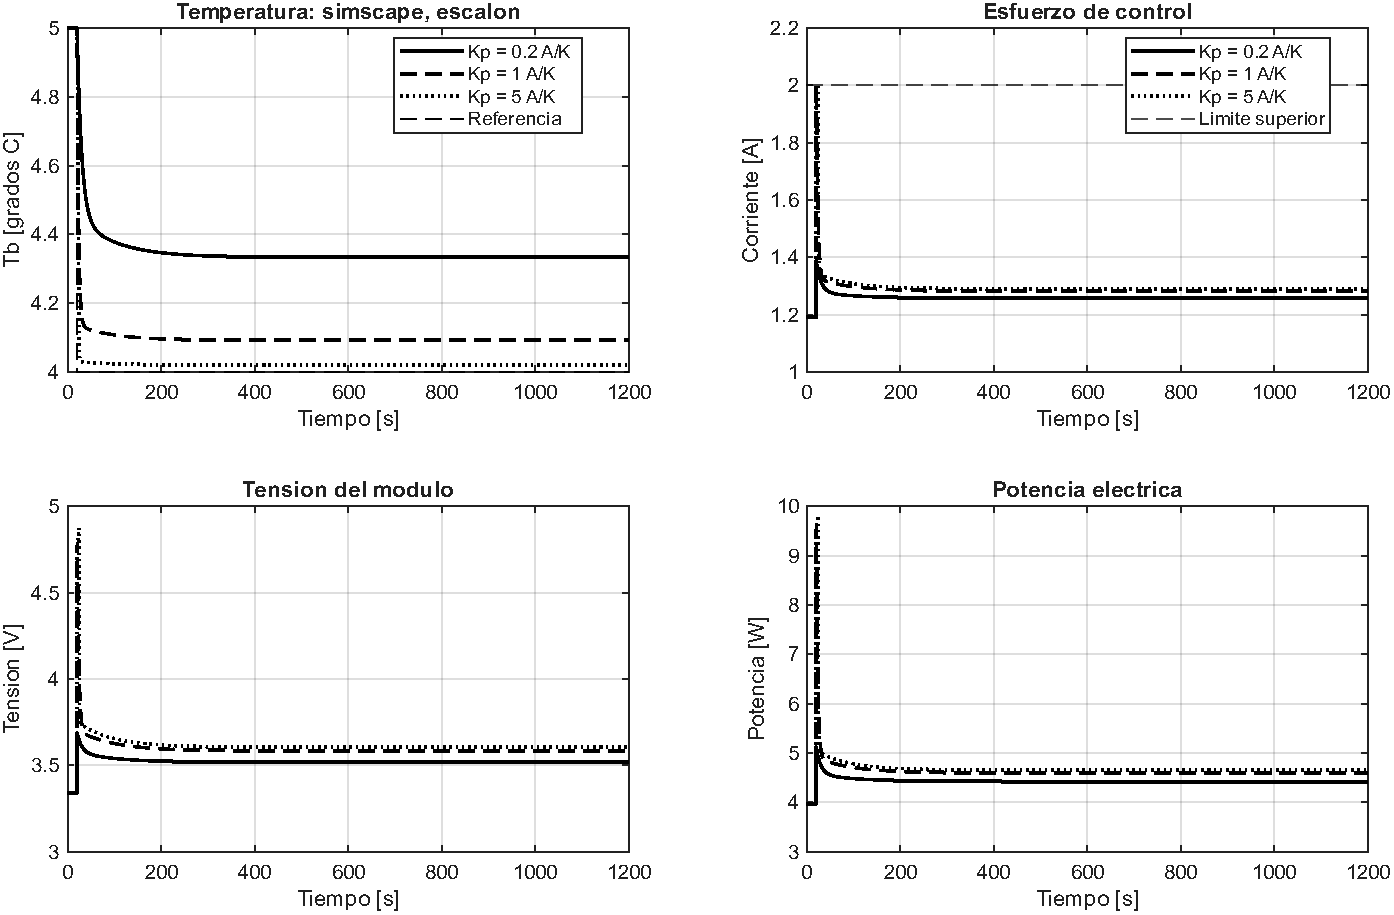
\includegraphics[width=\columnwidth]{../resultados_matlab/simscape_escalon.pdf}
\caption{Ensayo P de escalón, generado por la ejecución del modelo físico. Interpretar junto con \texttt{metricas\_P.csv}. Fuente: elaboración propia con MATLAB R2025a.}
\end{figure}
}{\pendiente{ejecutar los modelos nuevos en R2025a, verificar sus señales e incorporar las figuras y métricas realmente obtenidas.}}

La comparación definitiva debe incluir curvas de temperatura y corriente, las métricas y una interpretación por ensayo. El funcionamiento de los scripts y modelos nuevos no se certifica mediante la comprobación auxiliar.

% Responsable: Integrante 2 (tarea 2.2 del plan)
\section{Especificaciones de diseño}\label{sec:especificaciones}
Se considera que el bloque frío funciona como una pequeña cámara para conservar muestras o vacunas. La Organización Mundial de la Salud establece para su almacenamiento el rango de $+2$ a $+8\,^\circ\mathrm C$ \cite{who_pqs}; la referencia de $5\,^\circ\mathrm C$ queda en el centro de ese rango. Para la medición se supone un sensor digital DS18B20, con resolución de $0.0625\,^\circ\mathrm C$ en 12 bits y exactitud de $\pm0.5\,^\circ\mathrm C$ entre $-10$ y $+85\,^\circ\mathrm C$ \cite{ds18b20}. Con este contexto se definen las especificaciones de la Tabla~\ref{tab:especificaciones}. Las especificaciones E1 a E7 se evalúan con el modelo lineal alrededor del punto de operación ($T_{b0}=5\,^\circ\mathrm C$, $I_0=1.19\,\mathrm A$); la E8 se evalúa con el modelo no lineal.

\begin{table*}[!tbp]\centering
\caption{Especificaciones de diseño del lazo de temperatura.}\label{tab:especificaciones}
{\tableformat
\begin{tabularx}{\textwidth}{c>{\raggedright\arraybackslash}p{3.4cm}>{\raggedright\arraybackslash}p{5.2cm}L}\toprule
Id. & Métrica & Especificación & Justificación\\\midrule
E1 & Error en estado estable & $|e_{ss}|\le0.1\,\mathrm K$ para escalones de hasta $3\,\mathrm K$ & Equivale a menos de dos pasos de resolución del sensor \cite{ds18b20}. Un cambio de $3\,\mathrm K$ cubre toda la mitad del rango de $2$ a $8\,^\circ\mathrm C$ \cite{who_pqs}.\\
E2 & Sobrepaso & $M_p\le10\,\%$ & Para un escalón de $1\,\mathrm K$, el sobrepaso queda del mismo orden que la tolerancia de E1.\\
E3 & Tiempo de asentamiento (2\,\%) & $t_s\le180\,\mathrm s$ & Aproximadamente la mitad del tiempo de lazo abierto ($373\,\mathrm s$), para recuperar la temperatura después de abrir la cámara o introducir una muestra.\\
E4 & Esfuerzo de control en pequeña señal & $\Delta I_{\max}\le0.81\,\mathrm A$ ante un escalón de $-1\,\mathrm K$ & Con $I_0=1.19\,\mathrm A$, la corriente total no alcanza el límite de $2\,\mathrm A$ y el lazo trabaja sin saturar. La Tarea~1 mostró un error del modelo lineal cercano al $5\,\%$ con $|\Delta I|=1\,\mathrm A$.\\
E5 & Rango de la corriente & $0\le I\le2.0\,\mathrm A$ & Por debajo del mínimo de la curva estática ($2.42\,\mathrm A$, Figura~\ref{fig:limite}); la fuente no invierte la corriente.\\
E6 & Rechazo de perturbación & Escalón de $+5\,\mathrm K$ en $T_{\rm amb}$ o carga de $2\,\mathrm W$ en el bloque: pico $\le0.5\,\mathrm K$, regreso a $\pm0.1\,\mathrm K$ en $\le400\,\mathrm s$ y error final nulo & Un cambio de $25$ a $30\,^\circ\mathrm C$ en el ambiente es esperable durante el día, y la carga de $2\,\mathrm W$ representa introducir una muestra. En lazo abierto producirían $+4.6$ y $+5.0\,\mathrm K$, lo que saca al bloque del rango de $2$ a $8\,^\circ\mathrm C$.\\
E7 & Estabilidad relativa & Margen de fase $\ge45^\circ$ & Las masas del bloque y del disipador se marcaron como provisionales en la Tarea~1; el margen absorbe errores en esos parámetros.\\
E8 & Arranque desde $25\,^\circ\mathrm C$ (no lineal) & $T_b\ge2\,^\circ\mathrm C$ en todo momento y $|T_b-5\,^\circ\mathrm C|\le0.5\,\mathrm K$ antes de $300\,\mathrm s$ & No se aceptan temperaturas por debajo de $+2\,^\circ\mathrm C$ en el almacenamiento \cite{who_pqs}. Se exige además que el arranque sea más rápido que el de lazo abierto.\\\bottomrule
\end{tabularx}}
\par\smallskip\footnotesize Fuente: elaboración propia.
\end{table*}

Con las ecuaciones~\eqref{eq:essP} y \eqref{eq:essD} se ve que el control P no puede cumplir todas las especificaciones al mismo tiempo. La E1 exige $K_p\ge2.81\,\mathrm{A/K}$ y la E6 exige $K_p\ge4.35\,\mathrm{A/K}$ por la temperatura ambiente y $K_p\ge4.76\,\mathrm{A/K}$ por la carga de $2\,\mathrm W$, pero la E4 limita la ganancia a $K_p\le0.81\,\mathrm{A/K}$. Ningún valor de $K_p$ satisface las tres condiciones, por lo que se necesita un compensador.

% Responsable: Integrante 2 (tarea 2.3 del plan)
\section{Selección del compensador}\label{sec:seleccion}
El análisis anterior muestra que la deficiencia del control P está en el régimen permanente y en el rechazo de perturbaciones, no en el transitorio. Los polos de lazo cerrado son reales, no hay sobrepaso y, como se verá en la Sección~\ref{sec:diseno}, el margen de fase es amplio. La Tabla~\ref{tab:seleccion} compara las estructuras consideradas frente a estas deficiencias.

\begin{table}[!tbp]\centering
\caption{Comparación de estructuras de compensación para la planta de la ecuación~\eqref{eq:Gp}.}\label{tab:seleccion}
{\tableformat
\begin{tabularx}{\columnwidth}{lcL}\toprule
Estructura & $e_{ss}=0$ & Comentario\\\midrule
P & No & No cumple E1, E4 y E6 a la vez (Sección~\ref{sec:especificaciones}).\\
PD / adelanto & No & Mejoran la fase y la rapidez, que no son el problema. La acción derivativa amplifica los saltos de cuantización del sensor ($0.0625\,\mathrm K$).\\
Atraso & No & Reduce el error, pero no lo anula; requiere una ganancia en DC muy alta para cumplir E6.\\
PID & Sí & Cumple, pero la parte derivativa no aporta nada y agrega sensibilidad al ruido.\\
\textbf{PI} & \textbf{Sí} & El integrador vuelve el lazo tipo~1: error nulo ante escalones de referencia y de perturbación constante. Es la estructura más sencilla que corrige la deficiencia observada.\\\bottomrule
\end{tabularx}}
\par\smallskip\footnotesize Fuente: elaboración propia con base en \cite{ogata}.
\end{table}

Se selecciona un controlador PI. Su efecto esperado es agregar un polo en el origen, que anula el error permanente, y un cero real que se ubica para no hacer más lento el lazo. Como la planta ya tiene un margen de fase grande, la pérdida de fase que introduce el integrador a bajas frecuencias no compromete la estabilidad.

Por la limitación de la Sección~\ref{sec:limite}, la salida del PI se satura entre $0$ y $2\,\mathrm A$. Durante el arranque el error inicial es de $20\,\mathrm K$ y la corriente pasa cerca de $100\,\mathrm s$ saturada. Si el integrador sigue acumulando error en ese tiempo (\emph{windup}), al llegar a la referencia tiene un valor excesivo y el bloque se enfría de más. Por eso el PI se implementa con anti-windup por integración condicional (\emph{clamping}): la integral se congela mientras la salida está saturada \cite{astrom,mw_pid}.

% Responsable: Integrante 2 (tarea 2.4 del plan)
\section{Diseño del compensador}\label{sec:diseno}
\subsection{Estructura y ley de control}
El controlador PI se escribe como
\begin{equation}
C(s)=K_c\,\frac{s+z}{s}=K_c\left(1+\frac{1}{T_is}\right),\qquad z=\frac{1}{T_i},\label{eq:PI}
\end{equation}
y, en el dominio del tiempo, la corriente aplicada a la celda es
\begin{equation}
\begin{split}
I(t)&=\mathrm{sat}_{[0,\,2\,\mathrm A]}\Big\{I_0+K_c\,e(t)+K_i\!\int_0^t e(\tau)\,d\tau\Big\},\\
e(t)&=T_b(t)-T_{\rm ref},
\end{split}\label{eq:ley}
\end{equation}
con $K_i=K_c/T_i$. El término $I_0$ es la corriente del punto de operación y actúa como valor inicial de la salida. La Figura~\ref{fig:lazoPI} muestra cómo se implementa el lazo en Simulink.

\begin{figure}[!tbp]\centering
\begin{tikzpicture}[>=Latex,font=\footnotesize,
  bloque/.style={draw,thick,minimum height=8mm,minimum width=10mm,align=center},
  suma/.style={draw,thick,circle,inner sep=0pt,minimum size=4.5mm}]
\node (ref) at (0,0) {$T_{\rm ref}$};
\node[suma] (s1) at (1.15,0) {};
\node[bloque] (pi) at (2.65,0) {PI\\[-1pt]{\scriptsize $K_c,\,K_i$}\\[-1pt]{\scriptsize anti-windup}};
\node[suma] (s2) at (4.05,0) {};
\node (i0) at (4.05,0.95) {$I_0$};
\node[bloque] (sat) at (5.15,0) {\begin{tikzpicture}[scale=0.22]\draw (-1.4,-1)--(-0.7,-1)--(0.7,1)--(1.4,1);\end{tikzpicture}\\[-1pt]{\scriptsize 0--2 A}};
\node[bloque] (pl) at (6.95,0) {Planta\\[-1pt]{\scriptsize Simscape}};
\node (tamb) at (6.95,1.05) {$T_{\rm amb}$};
\node (y) at (8.15,0) {$T_b$};
\draw[->] (ref) -- node[pos=0.75,below]{$-$} (s1);
\draw[->] (s1) -- node[above]{$e$} (pi);
\draw[->] (pi) -- node[above]{$\Delta I$} (s2);
\draw[->] (i0) -- (s2);
\draw[->] (s2) -- (sat);
\draw[->] (sat) -- node[above]{$I$} (pl);
\draw[->] (tamb) -- (pl);
\draw[->] (pl) -- (y);
\draw[->] (7.75,0) -- (7.75,-0.95) -- node[below]{Sensor} (1.15,-0.95) -- node[pos=0.7,right]{$+$} (s1);
\end{tikzpicture}
\caption{Lazo de control con PI, saturación y anti-windup. El error se define como $e=T_b-T_{\rm ref}$ porque la planta tiene ganancia negativa. Fuente: elaboración propia.}\label{fig:lazoPI}
\end{figure}

\subsection{Ubicación del cero}
Los polos de la planta son $-0.0477$ y $-0.0086\,\mathrm{s^{-1}}$ (constantes de tiempo de $21$ y $116\,\mathrm s$). El polo lento domina la respuesta en lazo abierto. Si el integrador se agregara sin más, el polo en el origen y el polo lento formarían un par dominante muy lento. Por eso el cero del PI se coloca sobre el polo lento, de modo que lo cancele:
\begin{equation}
z=0.008607\,\mathrm{s^{-1}}\ \Rightarrow\ T_i=\frac{1}{z}=116.2\,\mathrm s.\label{eq:cero}
\end{equation}
Con esta cancelación, la ganancia de lazo abierto se reduce a
\begin{equation}
L(s)=C(s)G_p(s)=\frac{K_c\,(0.2919\,s+0.004243)}{s\,(s+0.04772)},\label{eq:L}
\end{equation}
y la ecuación característica del lazo cerrado queda
\begin{equation}
s^2+(0.04772+0.2919K_c)\,s+0.004243K_c=0.\label{eq:carPI}
\end{equation}
Igual que en la ecuación~\eqref{eq:carP}, todos los coeficientes son positivos para $K_c>0$, así que el lazo es estable para cualquier ganancia. El polo cancelado, $-0.0086\,\mathrm{s^{-1}}$, sigue presente en el lazo cerrado. No aparece en la respuesta a la referencia, pero sí en la respuesta a perturbaciones, como se discute más adelante.

\subsection{Selección de la ganancia}
Con el cero fijo, se calculó la respuesta del lazo para $0.1\le K_c\le1.5\,\mathrm{A/K}$ en pasos de $0.05$ (Figura~\ref{fig:barrido}). El tiempo de asentamiento disminuye con la ganancia y cumple la E3 a partir de $K_c=0.65\,\mathrm{A/K}$. El esfuerzo inicial vale $\Delta I(0^+)=K_c\,|\Delta T_{\rm ref}|$, por lo que la E4 limita la ganancia a $K_c\le0.81\,\mathrm{A/K}$. Dentro del intervalo $0.65\le K_c\le0.80\,\mathrm{A/K}$ se cumplen todas las especificaciones lineales. Se escoge un valor intermedio para dejar margen hacia ambos lados:
\begin{equation}
K_c=0.75\,\mathrm{A/K},\qquad K_i=\frac{K_c}{T_i}=6.456\times10^{-3}\,\mathrm{A/(K\,s)}.\label{eq:ganancias}
\end{equation}

\begin{figure}[!tbp]\centering
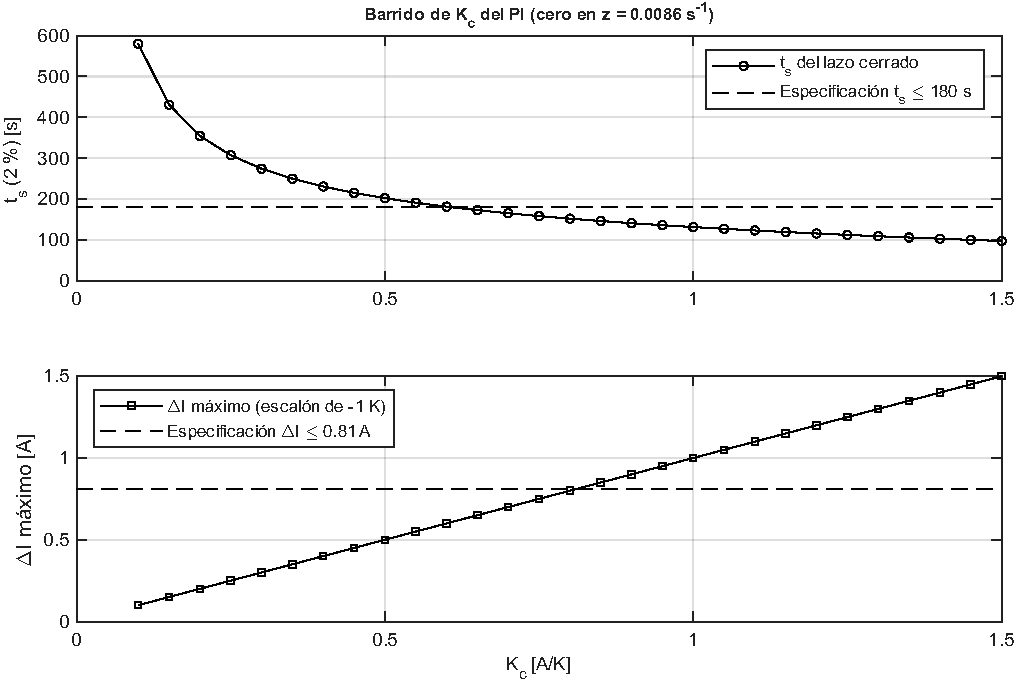
\includegraphics[width=\columnwidth]{barrido_Kc}
\caption{Tiempo de asentamiento y esfuerzo de control máximo en función de $K_c$, con el cero del PI fijo en $z=0.0086\,\mathrm{s^{-1}}$. Las líneas discontinuas son las especificaciones E3 y E4. Fuente: elaboración propia con MATLAB R2025a.}\label{fig:barrido}
\end{figure}

Al sustituir $K_c=0.75\,\mathrm{A/K}$ en la ecuación~\eqref{eq:carPI} se obtienen los polos de lazo cerrado $-0.2541$ y $-0.0125\,\mathrm{s^{-1}}$, a los que se suma el polo cancelado en $-0.0086\,\mathrm{s^{-1}}$. La Figura~\ref{fig:lgrPI} los ubica sobre el lugar de las raíces. El polo en $-0.0125\,\mathrm{s^{-1}}$ queda muy cerca del cero en $-0.0145\,\mathrm{s^{-1}}$, por lo que su aporte a la respuesta es pequeño y la salida se acerca rápido a la referencia.

\begin{figure}[!tbp]\centering
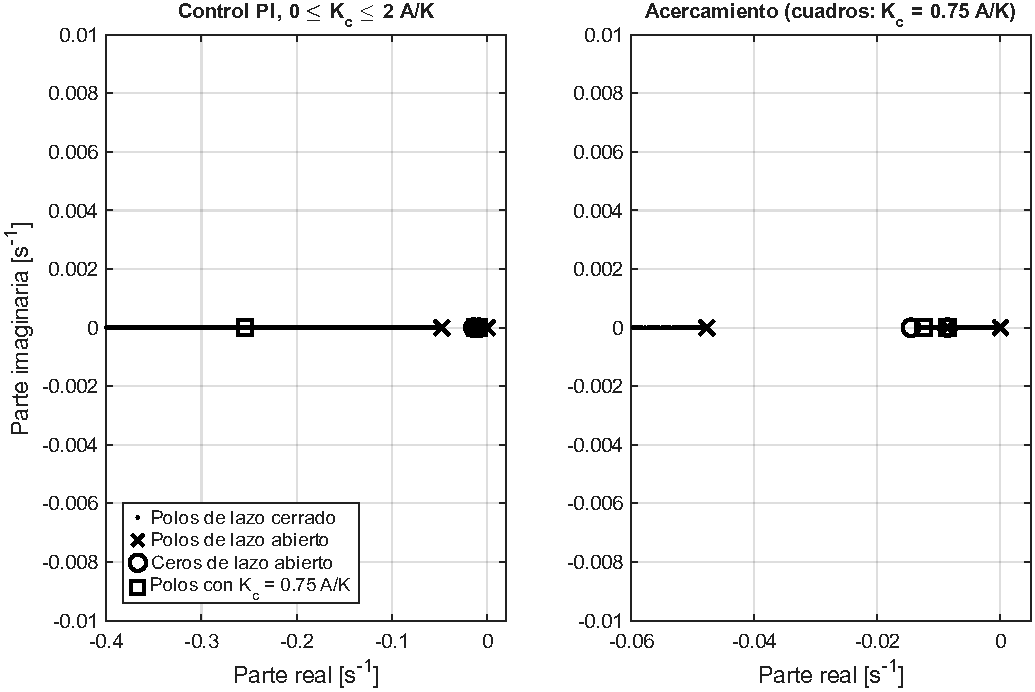
\includegraphics[width=\columnwidth]{lgr_PI}
\caption{Lugar de las raíces de $K_c(s+z)G_p(s)/s$ para $0\le K_c\le2\,\mathrm{A/K}$; los cuadrados son los polos con $K_c=0.75\,\mathrm{A/K}$. Fuente: elaboración propia con MATLAB R2025a.}\label{fig:lgrPI}
\end{figure}

\subsection{Verificación en frecuencia}
La Figura~\ref{fig:bode} muestra el diagrama de Bode de $L(s)$. El margen de fase es de $98.7^\circ$ a $0.214\,\mathrm{rad/s}$ y el margen de ganancia es infinito, porque la fase nunca llega a $-180^\circ$. Se cumple la E7 con amplitud.

\begin{figure}[!tbp]\centering
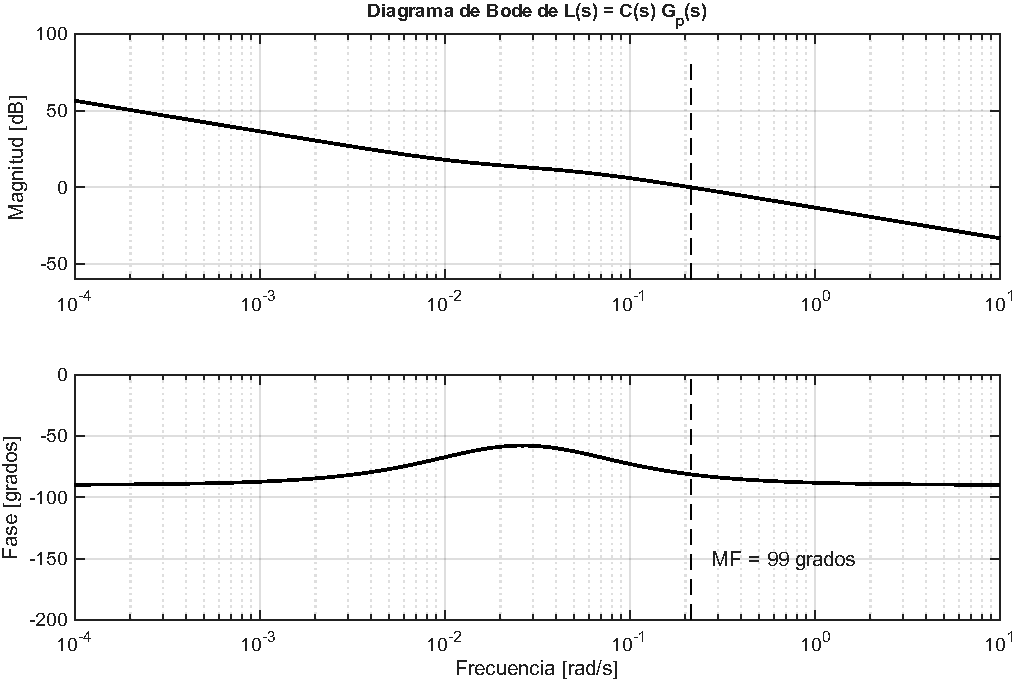
\includegraphics[width=\columnwidth]{bode_PI}
\caption{Diagrama de Bode de la ganancia de lazo $L(s)=C(s)G_p(s)$ con $K_c=0.75\,\mathrm{A/K}$ y $T_i=116.2\,\mathrm s$. La línea discontinua marca la frecuencia de cruce de ganancia. Fuente: elaboración propia con MATLAB R2025a.}\label{fig:bode}
\end{figure}

\subsection{Comprobación con el modelo no lineal}
Para respaldar la elección del límite de corriente y del anti-windup se integró el modelo no lineal de la Tarea~1 con el método de Euler (paso de $0.05\,\mathrm s$) durante un arranque desde $25\,^\circ\mathrm C$ con $T_{\rm ref}=5\,^\circ\mathrm C$ (Figura~\ref{fig:arranque}). Con límite de $6.4\,\mathrm A$, la corriente se queda en el máximo y el bloque se calienta hasta $46.4\,^\circ\mathrm C$. Con límite de $2\,\mathrm A$ pero sin anti-windup, el integrador acumula error durante la saturación y el bloque baja hasta $1.92\,^\circ\mathrm C$, lo que viola la E8. Con el diseño completo, la temperatura mínima es $4.87\,^\circ\mathrm C$ y el bloque entra a la banda de $5\pm0.5\,^\circ\mathrm C$ a los $117\,\mathrm s$. La validación formal se hace con la red de Simscape en la Sección~\ref{sec:resultados}.

\begin{figure}[!tbp]\centering
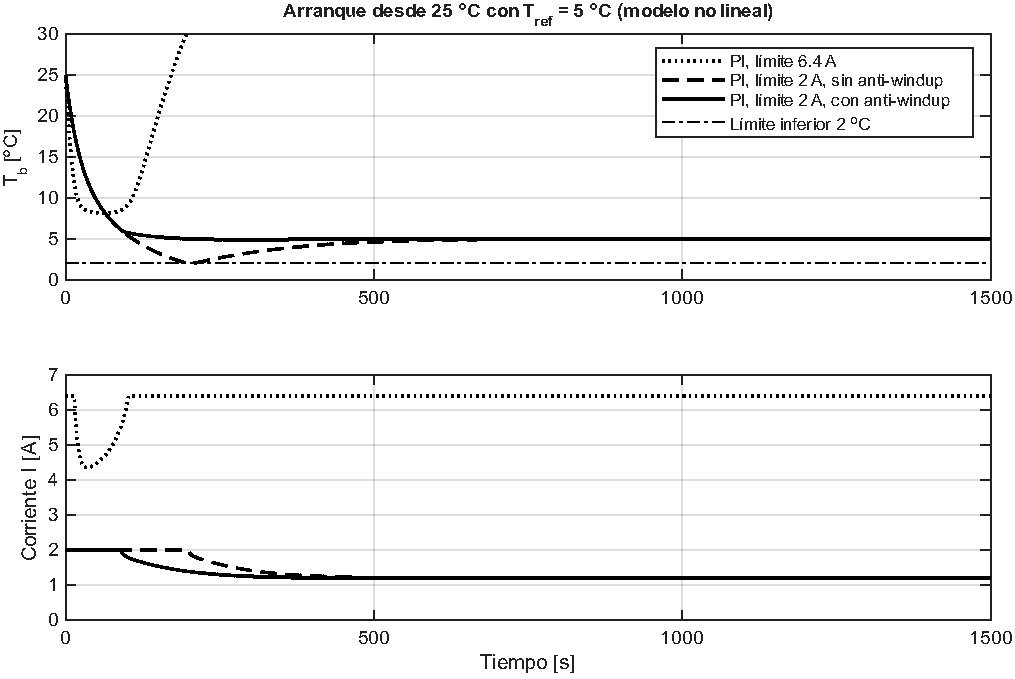
\includegraphics[width=\columnwidth]{arranque_nl}
\caption{Arranque desde $25\,^\circ\mathrm C$ con el modelo no lineal para tres implementaciones del PI ($K_c=0.75\,\mathrm{A/K}$, $T_i=116.2\,\mathrm s$). Fuente: elaboración propia con MATLAB R2025a.}\label{fig:arranque}
\end{figure}

\subsection{Resumen del diseño}
La Figura~\ref{fig:escalonPPI} compara el P y el PI con la misma ganancia proporcional ($0.75\,\mathrm{A/K}$) ante un escalón de referencia de $-1\,\mathrm K$, con el modelo lineal. El P se queda a $0.11\,\mathrm K$ de la referencia, mientras que el PI la alcanza; la corriente de ambos arranca en $0.75\,\mathrm A$, dentro de la E4.

\begin{figure}[!tbp]\centering
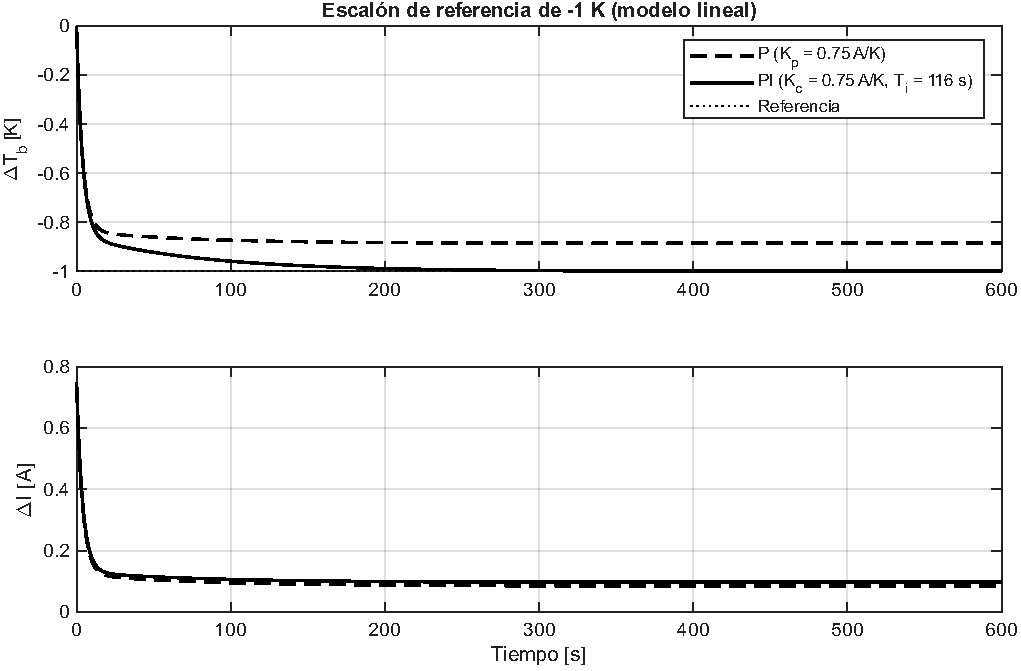
\includegraphics[width=\columnwidth]{escalon_P_PI}
\caption{Respuesta lineal a un escalón de referencia de $-1\,\mathrm K$ con control P ($K_p=0.75\,\mathrm{A/K}$) y con el PI diseñado: desviación de la temperatura (arriba) y de la corriente (abajo). Fuente: elaboración propia con MATLAB R2025a.}\label{fig:escalonPPI}
\end{figure}

La Figura~\ref{fig:pertPPI} muestra las dos perturbaciones de la E6. En lazo abierto el bloque se desvía $4.6$ y $5.0\,\mathrm K$; con el P la desviación permanente baja a cerca de $0.5\,\mathrm K$, y con el PI el pico es de $0.26$ y $0.30\,\mathrm K$ y la desviación vuelve a cero.

\begin{figure}[!tbp]\centering
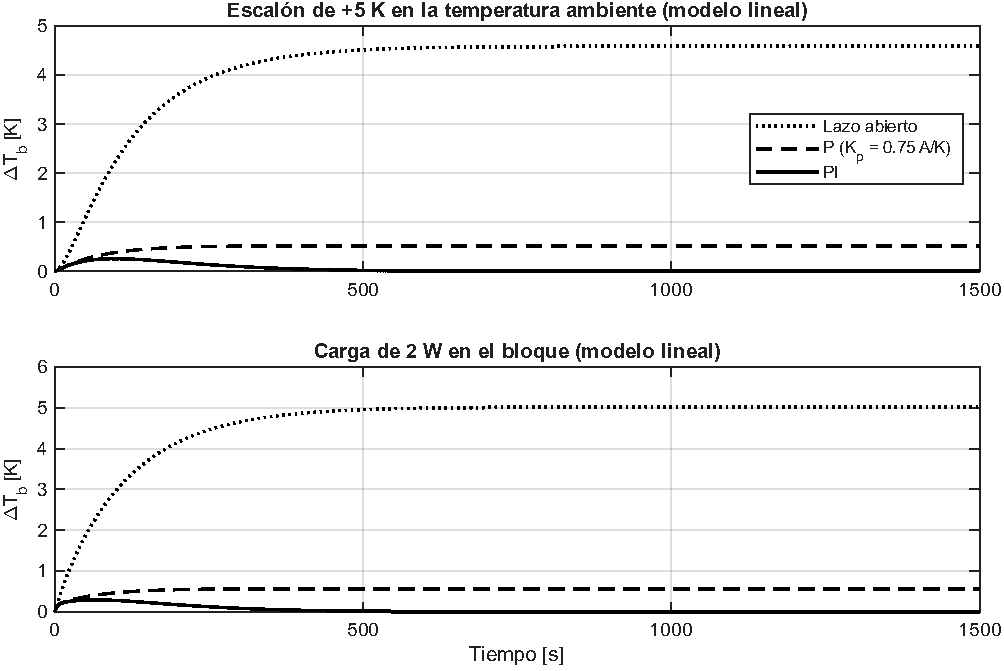
\includegraphics[width=\columnwidth]{perturbacion_P_PI}
\caption{Respuesta lineal a un escalón de $+5\,\mathrm K$ en la temperatura ambiente (arriba) y a una carga de $2\,\mathrm W$ en el bloque (abajo), en lazo abierto, con control P y con el PI. Fuente: elaboración propia con MATLAB R2025a.}\label{fig:pertPPI}
\end{figure}

La Tabla~\ref{tab:prediccion} compara el desempeño previsto del diseño con las especificaciones de la Tabla~\ref{tab:especificaciones}. Todas se cumplen. Para la implementación en el bloque \emph{PID Controller} de Simulink se usa la forma paralela con $P=K_c$, $I=K_i$ y $D=0$, saturación de salida y anti-windup por \emph{clamping} \cite{mw_pid}. Los valores se guardan en \texttt{parametros\_control.mat}.

\begin{table}[!htbp]\centering
\caption{Desempeño previsto del PI frente a las especificaciones.}\label{tab:prediccion}
{\tableformat
\begin{tabular}{clccc}\toprule
Id. & Métrica & Especificación & PI diseñado & ¿Cumple?\\\midrule
E1 & $e_{ss}$ & $\le0.1\,\mathrm K$ & $0$ & Sí\\
E2 & $M_p$ & $\le10\,\%$ & $0\,\%$ & Sí\\
E3 & $t_s$ (2\,\%) & $\le180\,\mathrm s$ & $158.6\,\mathrm s$ & Sí\\
E4 & $\Delta I_{\max}$ ($-1\,\mathrm K$) & $\le0.81\,\mathrm A$ & $0.75\,\mathrm A$ & Sí\\
E5 & Rango de $I$ & $0$ a $2\,\mathrm A$ & $0$ a $2\,\mathrm A$ & Sí\\
E6 & Pico / regreso & $\le0.5\,\mathrm K$ / $\le400\,\mathrm s$ & $0.30\,\mathrm K$ / $300\,\mathrm s$ & Sí\\
E7 & Margen de fase & $\ge45^\circ$ & $98.7^\circ$ & Sí\\
E8 & $T_{b,\min}$ / $t_{\pm0.5}$ & $\ge2\,^\circ\mathrm C$ / $\le300\,\mathrm s$ & $4.87\,^\circ\mathrm C$ / $117\,\mathrm s$ & Sí\\\bottomrule
\end{tabular}}
\par\smallskip\footnotesize Fuente: elaboración propia. E1 a E7 con el modelo lineal; E8 con el modelo no lineal. En E6 se reporta el peor caso: pico de $0.26\,\mathrm K$ por $T_{\rm amb}$ y de $0.30\,\mathrm K$ por la carga de $2\,\mathrm W$.
\end{table}

% Responsable: Integrante 3 (tarea 3.4 del plan)
% Usar peltier_lazo_comp.slx con parametros_control.mat (Kc, Ki, numC, denC),
% saturación de 0 a 2 A y anti-windup Clamping. Mismas pruebas que el
% integrante 1: escalón de -1 K, arranque desde 25 C, carga de 2 W y ruido.
\section{Resultados de simulación}\label{sec:resultados}
\pendiente{respuestas del sistema compensado en Simscape (temperatura y corriente) para el escalón de referencia, el arranque, la carga de $2\,\mathrm W$ y el ruido, cada figura con su interpretación. Comparar con las predicciones lineales de las Figuras~\ref{fig:escalonPPI} y~\ref{fig:pertPPI}.}

% Responsable: Integrante 3 (tarea 3.5 del plan). Verificación: Integrante 2.
% Llenar las columnas P y compensado con las métricas de Simscape
% (metricas_lazo.m). La columna de especificación ya está completa.
\section{Análisis comparativo}\label{sec:comparacion}
La Tabla~\ref{tab:comparacion} compara el control proporcional con el sistema compensado frente a las especificaciones de la Tabla~\ref{tab:especificaciones}. \pendiente{discusión de cada métrica y de si se cumplen las especificaciones.}

\begin{table}[!tbp]\centering
\caption{Comparación cuantitativa entre el control P y el sistema compensado.}\label{tab:comparacion}
{\tableformat
\begin{tabular}{@{}lccc@{}}\toprule
Métrica & Especificación & Control P & Compensado\\\midrule
Error en estado estable & $\le0.1\,\mathrm K$ & -- & --\\
Tiempo de asentamiento & $\le180\,\mathrm s$ & -- & --\\
Tiempo de subida & -- & -- & --\\
Sobrepaso & $\le10\,\%$ & -- & --\\
Esfuerzo de control máximo & $\le0.81\,\mathrm A$ ($-1\,\mathrm K$) & -- & --\\
Pico por carga de 2\,W & $\le0.5\,\mathrm K$ & -- & --\\
Estabilidad (MF) & $\ge45^\circ$ & -- & --\\
Arranque: $T_{b,\min}$ & $\ge2\,^\circ\mathrm C$ & -- & --\\\bottomrule
\end{tabular}}
\par\smallskip\footnotesize Fuente: elaboración propia con MATLAB R2025a.
\end{table}

% Responsables: Integrante 1 (sensibilidad, tarea 1.6) e Integrante 2
% (compromisos de diseño, tarea 2.6)
\section{Discusión}\label{sec:discusion}
\subsection{Sensibilidad paramétrica y limitaciones}\label{sec:sensibilidad}
Se preparó la repetición del escalón nominal variando $R_{HA}$ entre $1.29$, $2.11$ y $8.4\,\mathrm{K/W}$, la masa fría en $\pm20\%$ y el punto de operación a $10\,{}^\circ\mathrm C$. Se mantienen las ganancias. Para el cambio de masa se conserva la resistencia térmica y se modifica la capacidad de almacenamiento; para el punto de $10\,{}^\circ\mathrm C$ se recalcula el sesgo de equilibrio de ambos controladores y se usa un escalón de $10$ a $9\,{}^\circ\mathrm C$.

Antes de atribuir diferencias al controlador se evaluó la factibilidad estática con los balances de la planta. Un barrido de corrientes de $0$ a $6.4\,\mathrm A$, con paso de $0.001\,\mathrm A$, produjo los mínimos aproximados de la Tabla~\ref{tab:factibilidad}. Se excluyeron equilibrios inestables y temperaturas absolutas no físicas.

\begin{table}[!tbp]\centering
\caption{Factibilidad calculada con el modelo térmico de Tarea 1.}
\label{tab:factibilidad}
\footnotesize
\begin{tabular}{@{}ccc@{}}\toprule
Disipación&$T_{b,\min}$ [$^\circ$C]&Corriente [A]\\\midrule
400 LFM&$-1.053$&2.421\\
200 LFM&6.710&1.681\\
Natural&20.146&0.495\\\bottomrule
\end{tabular}
\par\smallskip\footnotesize Fuente: elaboración propia.
\end{table}
Según estas hipótesis, $5\,{}^\circ\mathrm C$ no es un equilibrio alcanzable con 200 LFM ni con convección natural. Un compensador no elimina esta restricción física. En tales casos deben discutirse saturación, rechazo térmico y validez de las temperaturas predichas, en lugar de exigir cumplimiento de una referencia imposible.

El estudio P está programado y se dispone de una referencia auxiliar de las ecuaciones. La ley de control compensada ya está definida (Sección~\ref{sec:diseno}); la repetición de estos casos con el PI queda condicionada al modelo compensado del integrante 3. \pendiente{resultados de sensibilidad con P y con PI.}

\subsection{Compromisos de diseño}\label{sec:compromisos}
La ganancia $K_c$ concentra el principal compromiso del diseño. Un valor mayor acelera la respuesta y reduce el pico ante perturbaciones (Figura~\ref{fig:barrido}), pero exige más corriente, satura antes y amplifica el ruido de cuantización del sensor: cada paso de $0.0625\,\mathrm K$ produce un salto de $K_c\times0.0625\approx0.05\,\mathrm A$ en la corriente. El límite de $2\,\mathrm A$ también es un compromiso, porque protege el lazo contra la inversión de la ganancia a costa de no aprovechar toda la capacidad de enfriamiento de la celda.

La cancelación del polo lento hace que la respuesta a la referencia sea rápida ($158.6\,\mathrm s$), pero deja ese polo en la respuesta a perturbaciones, que tarda $300\,\mathrm s$ en volver a $\pm0.1\,\mathrm K$. Además, la cancelación depende de los parámetros: el polo de $-0.0086\,\mathrm{s^{-1}}$ cambia con la resistencia del disipador y con las masas, que siguen siendo provisionales. Si la cancelación no es exacta, aparece un par polo--cero cercano que agrega una cola lenta de poca amplitud, pero no compromete la estabilidad, porque la ecuación~\eqref{eq:carPI} tiene coeficientes positivos para cualquier $K_c$. El efecto de estas variaciones se cuantifica en la Sección~\ref{sec:sensibilidad}.

El límite de $2\,\mathrm A$ se eligió con el disipador ventilado a $400\,\mathrm{LFM}$. Si el ventilador falla, el mínimo de la curva estática se desplaza a corrientes menores y queda por encima de $5\,^\circ\mathrm C$ (Tabla~\ref{tab:factibilidad}). En esos casos la referencia de $5\,^\circ\mathrm C$ es inalcanzable con cualquier controlador, el integrador lleva la corriente al límite y, en convección natural, el equilibrio con $2\,\mathrm A$ queda en $63\,^\circ\mathrm C$. Por eso el sistema real necesita detectar la falla del ventilador, por ejemplo con la temperatura del lado caliente, y reducir la corriente. Como mejoras futuras se proponen una prealimentación de la temperatura ambiente para acelerar el rechazo de perturbaciones y un límite de corriente que dependa de la temperatura del lado caliente.

% Responsables: los tres. Cerrar después de tener los resultados de Simscape.
\section{Conclusiones}\label{sec:conclusiones}
El control P reduce el error local al aumentar la ganancia, con los compromisos de esfuerzo y ruido que deben cuantificarse en las pruebas. La estabilidad lineal nominal no asegura el arranque del sistema físico saturado. La comprobación auxiliar advirtió un fallo de arranque para las dos ganancias mayores con el límite de $6.4\,\mathrm A$, explicado por la inversión de la ganancia de la planta por encima de $2.42\,\mathrm A$. Además, la sensibilidad de la disipación revela límites de factibilidad que requieren distinguir el diseño de control del dimensionamiento térmico.

Ningún valor de $K_p$ cumple a la vez las especificaciones de error, de rechazo de perturbaciones y de esfuerzo de control. Un PI con el cero sobre el polo lento de la planta, $K_c=0.75\,\mathrm{A/K}$, salida limitada a $2\,\mathrm A$ y anti-windup cumple las ocho especificaciones en el modelo lineal y en la comprobación no lineal del arranque. \pendiente{confirmar con Simscape y cerrar con la comparación de la Tabla~\ref{tab:comparacion}.}


\balance
% Referencias. Las de la Tarea 1 que aún no se citan están comentadas al final:
% descomentarlas cuando el integrante 3 las use en la descripción del sistema.
\begin{thebibliography}{10}
\bibitem{hb} HB Corporation, \emph{Thermoelectric Cooler TEC1-12706}, rev. 2.03, pp. 1--3.
\bibitem{who_pqs} World Health Organization, \emph{WHO PQS: Vaccine and immunization devices -- Terms and definitions}, definición de \emph{acceptable temperature range}. [En línea]. Disponible: \url{https://extranet.who.int/prequal/key-resources/documents/who-vax-imd-terms-definitions}. Consultado: nov. 2026.
\bibitem{ds18b20} Maxim Integrated (Analog Devices), \emph{DS18B20: Programmable Resolution 1-Wire Digital Thermometer}, hoja de datos. [En línea]. Disponible: \url{https://www.analog.com/en/products/ds18b20.html}. Consultado: nov. 2026.
\bibitem{ogata} K. Ogata, \emph{Ingeniería de control moderna}, 5.ª ed. Madrid, España: Pearson Educación, 2010.
\bibitem{astrom} K. J. Åström y T. Hägglund, \emph{Advanced PID Control}. Research Triangle Park, NC, EE.\,UU.: ISA, 2006.
\bibitem{mw_pid} MathWorks, \emph{PID Controller}, Simulink. [En línea]. Disponible: \url{https://www.mathworks.com/help/simulink/slref/pidcontroller.html}. Consultado: nov. 2026.
% \bibitem{wakefielddatasheet} Wakefield-Vette, \emph{Elliptical Fin Heat Sink: 900 Series}, tabla de rendimiento térmico y sistema de numeración de partes.
% \bibitem{tme} TME, \emph{910-40-1-23-2-B-0 Wakefield Thermal -- Heatsink: extruded}. [En línea]. Disponible: \url{https://www.tme.eu/en/details/910-40-1-23-2-b-0/heatsinks/wakefield-thermal/}. Consultado: oct. 2026.
% \bibitem{digikey} DigiKey, \emph{Wakefield Thermal Solutions 910-40-1-23-2-B-0}. [En línea]. Disponible: \url{https://www.digikey.com/en/products/detail/wakefield-thermal-solutions/910-40-1-23-2-B-0/4815169}. Consultado: sep. 2026.
% \bibitem{gonzales} R. D. Gonzales Toledo, \emph{Sistema de refrigeración con efecto Peltier y superficies extendidas, para enfriamiento sensible de aire}, tesis de maestría, Pontificia Universidad Católica del Perú, 2018. [En línea]. Disponible: \url{https://tesis.pucp.edu.pe/server/api/core/bitstreams/65ed2cce-ed4d-484a-bac4-94b46bb1cc59/content}
% \bibitem{ferrotec} Ferrotec, \emph{Thermoelectric Reference Guide: Mathematical Modeling of Modules}, secs. 11.2, 11.4 y 11.6. [En línea]. Disponible: \url{https://thermal.ferrotec.com/technology/thermoelectric-reference-guide/thermalref11/}. Consultado: sep. 2026.
% \bibitem{mw_peltier} MathWorks, \emph{Peltier Device}, Simscape Electrical. [En línea]. Disponible: \url{https://www.mathworks.com/help/simscape-electrical/ref/peltierdevice.html}. Consultado: oct. 2026.
% \bibitem{mw_mass} MathWorks, \emph{Thermal Mass}, Simscape Foundation Library. [En línea]. Disponible: \url{https://www.mathworks.com/help/simscape/ref/thermalmass.html}. Consultado: oct. 2026.
% \bibitem{mw_resistance} MathWorks, \emph{Thermal Resistance}, Simscape Foundation Library. [En línea]. Disponible: \url{https://www.mathworks.com/help/simscape/ref/thermalresistance.html}. Consultado: oct. 2026.
% \bibitem{mw_heat} MathWorks, \emph{Controlled Heat Flow Rate Source}, Simscape Foundation Library. [En línea]. Disponible: \url{https://www.mathworks.com/help/simscape/ref/controlledheatflowratesource.html}. Consultado: oct. 2026.
\end{thebibliography}

\end{document}
